\documentclass{article}

\usepackage{amsmath, amsthm, amssymb, amsfonts}
\usepackage{thmtools}
\usepackage{graphicx}
\usepackage{setspace}
\usepackage{geometry}
\usepackage{float}
\usepackage{hyperref}
\usepackage[utf8]{inputenc}
\usepackage[english]{babel}
\usepackage{framed}
\usepackage[dvipsnames]{xcolor}
\usepackage{tcolorbox}

\colorlet{LightGray}{White!90!Periwinkle}
\colorlet{LightOrange}{Orange!15}
\colorlet{LightGreen}{Green!15}

\newcommand{\HRule}[1]{\rule{\linewidth}{#1}}

\declaretheoremstyle[name=Theorem,]{thmsty}
\declaretheorem[style=thmsty,numberwithin=section]{theorem}
\tcolorboxenvironment{theorem}{colback=LightGray}

\declaretheoremstyle[name=Proposition,]{prosty}
\declaretheorem[style=prosty,numberlike=theorem]{proposition}
\tcolorboxenvironment{proposition}{colback=LightOrange}

\declaretheoremstyle[name=Principle,]{prcpsty}
\declaretheorem[style=prcpsty,numberlike=theorem]{principle}
\tcolorboxenvironment{principle}{colback=LightGreen}

\setstretch{1.2}
\geometry{
    textheight=9in,
    textwidth=5.5in,
    top=1in,
    headheight=12pt,
    headsep=25pt,
    footskip=30pt
}

% ------------------------------------------------------------------------------

\begin{document}

% ------------------------------------------------------------------------------
% Cover Page and ToC
% ------------------------------------------------------------------------------

\title{ \normalsize \textsc{}
\\ [2.0cm]
\HRule{1.5pt} \\
\LARGE \textbf{\uppercase{Documento de Casos de Uso}
\HRule{2.0pt} \\ [0.6cm] \LARGE{Inventario del Cuarto} \vspace*{10\baselineskip}}
}
\date{}
\author{\textbf{Ricardo Emmanuel Uriegas Ibarra}}

\maketitle
% remove page number from the cover page
\thispagestyle{empty} % Quita el número de página en esta página
\newpage

\tableofcontents
\newpage

% ------------------------------------------------------------------------------

\section{Introduction}
\subsection{Propósito del Documento}
Este documento tiene como objetivo describir los requisitos funcionales y no funcionales del \textit{Sistema de Inventario del Cuarto}. Los requisitos aquí documentados son el resultado de entrevistas y validaciones con el cliente; con el propósito de asegurar cubre las necesidades correspondientes.

\subsection{Alcance del Sistema}
El sistema permitira gestionar de mejor manera el inventario de items del dormitorio. La solucion proposiona una interfaz moderna y amigable para el usuario.

\section{Requisitos Funcionales}
\subsection{RF1. Gestionar Items}
\begin{itemize}
	\item Descripción: El sistema permitirá al usuario agregar, modificar y eliminar items del inventario.
	\item Regla: El usuario debe estar autenticado para realizar esta acción.
\end{itemize}

\subsection{RF2. Gestionar Inmuebles}
\begin{itemize}
	\item Descripción: El sistema permitirá al usuario agregar, modificar y eliminar inmuebles.
	\item Regla: El usuario debe estar autenticado para realizar esta acción.
\end{itemize}

\subsection{RF3. Gestionar Muebles}
\begin{itemize}
	\item Descripción: El sistema permitirá al usuario agregar, modificar y eliminar muebles.
	\item Regla: El usuario debe estar autenticado para realizar esta acción.
\end{itemize}

\subsection{RF4. Autenticación}
\begin{itemize}
    \item Descripción: El sistema permitirá al usuario autenticarse.
    \item Regla: El usuario debe ingresar una contraseña válida definida con anterioridad.
\end{itemize}


\section{Requisitos No Funcionales}
\subsection{RFN1. Usabilidad}
\begin{itemize}
    \item Descripción: La interfaz de usuario debe ser amigable y fácil de usar.
    \item Regla: La interfaz debe ser intuitiva y fácil de usar.
\end{itemize}

\subsection{RFN2. Seguridad}
\begin{itemize}
    \item Descripción: El sistema debe ser seguro.
    \item Regla: La información del usuario debe ser encriptada.
\end{itemize}

\subsection{RFN3. Rendimiento}
\begin{itemize}
    \item Descripción: El sistema debe ser rápido.
    \item Regla: El sistema debe responder en menos de 5 segundos debido a que se mantiene de manera local.
\end{itemize}

\section{Casos de Uso}

\section{Riesgos Identificados}

\section{Aprobación del Documento}

\section{Conclusion}

\section{Anexos}

%%%%%%%%%%%%%%%%%%%%%%%%%%%%%%%%%%%%%%%%%%%%%%%
\newpage
\section{Examples}

\begin{theorem}
	This is a theorem.
\end{theorem}

\begin{proposition}
	This is a proposition.
\end{proposition}

\begin{principle}
	This is a principle.
\end{principle}

% Maybe I need to add one more part: Examples.
% Set style and colour later.

\subsection{Pictures}

\begin{figure}[htbp]
	\center
	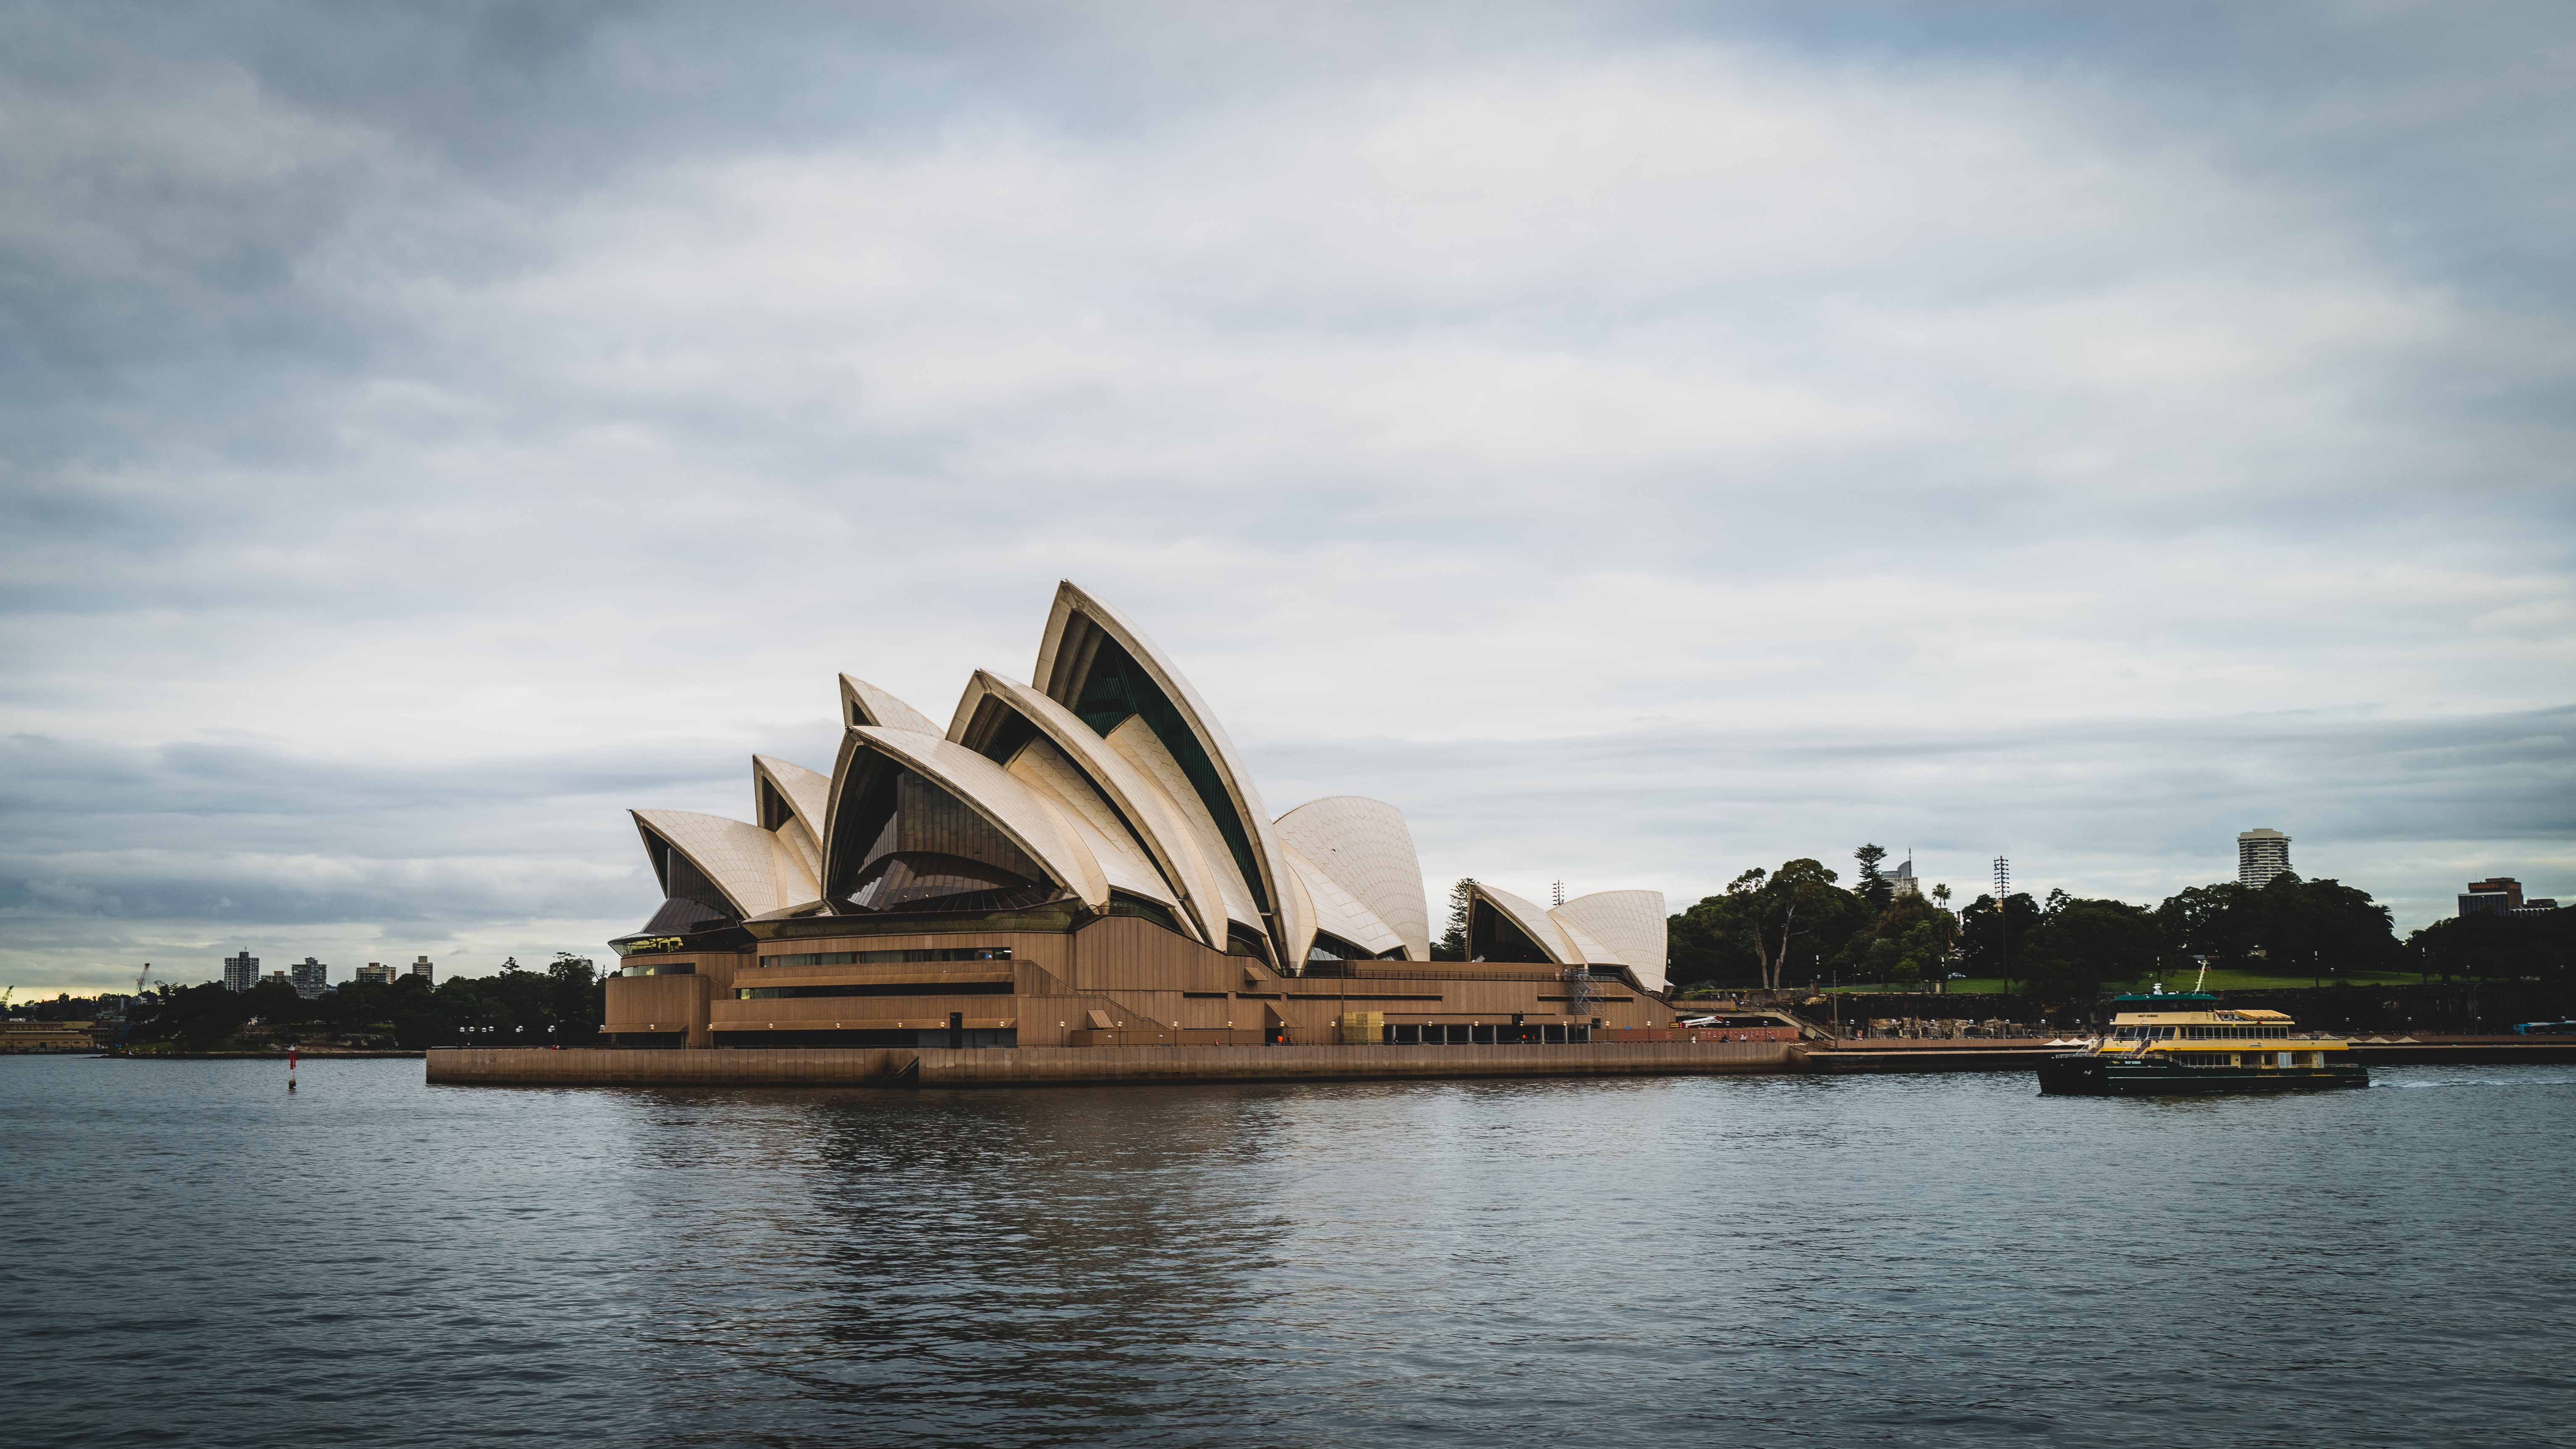
\includegraphics[scale=0.06]{img/photo.jpg}
	\caption{Sydney, NSW}
\end{figure}

\subsection{Citation}

This is a citation\cite{Eg}.

\newpage

% ------------------------------------------------------------------------------
% Reference and Cited Works
% ------------------------------------------------------------------------------

\bibliographystyle{IEEEtran}
\bibliography{References.bib}

% ------------------------------------------------------------------------------

\end{document}
